\chapter{MÔ HÌNH ĐỀ XUẤT}
\section{Mô hình}
\subsection{Mô hình nhận diện khuôn mặt}
Mô hình nhận diện khuôn mặt sử dụng giải thuật Facial Landmarks. Trong khi giải thuật gốc vẽ ra 81 điểm mốc bao quanh khuôn mặt, mô hình lược bỏ một số điểm mốc nhận diện mắt, mũi, môi, còn lại 30 điểm mốc bao quanh khuôn mặt như thể hiện ở hình~\ref{fig:Facial_Landmarks}.

\begin{figure}[ht]
    \centering
    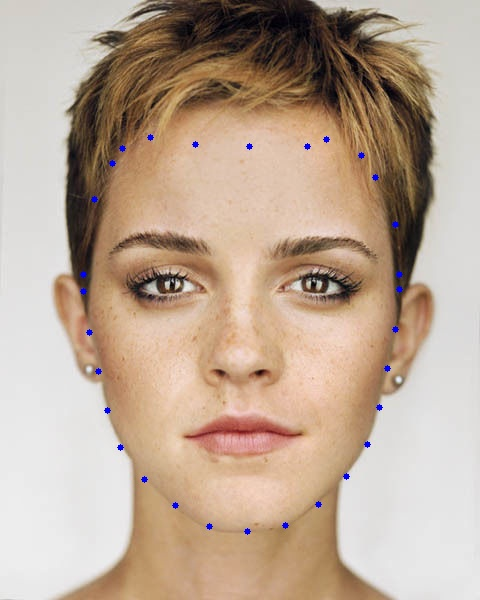
\includegraphics[width=5cm]{Images/Facial_Landmarks.jpg}
    \caption[Kết quả mô hình nhận diện khuôn mặt]
    {Kết quả mô hình nhận diện khuôn mặt với 30 điểm mốc}
    \label{fig:Facial_Landmarks}
\end{figure}
% \newpage
Căn cứ vào 30 điểm mốc bao quanh khuôn mặt, đề tài sử dụng công thức tính tỉ lệ khuôn mặt như sau:
\begin{equation}
R_{f} = \frac{N_{f}}{N}\\
\end{equation}
Với $N_{f}$ được tính bởi công thức~\ref{equa:polygon_area}, trong đó $(x_{n},y_{n})$ là tọa độ các điểm mốc được nhận dạng trên ảnh:
\begin{equation}
N_{f} = \sum_{1}^{n=30} \frac{\abs{(x_{1}y_{2} - y_{1}x_{2}) + (x_{2}y_{3} - y_{2}x_{3}) + ... + (x_{n}y_{1} - y_{n}x_{1})}}{2}\\
\label{equa:polygon_area}
\end{equation}
Trong đó:
\begin{itemize}[noitemsep]
\addtolength{\itemindent}{1.5cm}
    \item $R_{f}$: tỉ lệ khuôn mặt trên toàn bộ bức ảnh\\
    \item $N_{f}$: tổng diện tích khuôn mặt lọc bởi mô hình\\
    \item N: kích thước tấm ảnh
\end{itemize}
Tuy nhiên, mô hình nhận diện khuôn mặt vẫn có một số hạn chế khi thực nghiệm trên những khuôn mặt mờ hoặc xuất hiện không đầy đủ, thậm chí là những tấm ảnh chụp nghiêng. Những nhược điểm này sẽ được tìm cách khắc phục trong những công trình nghiên cứu sau.